% Provenance (never printed): cycle 3 geography and "La planete Terre"
% (the great physical features of the world: relief, rivers, deserts, ice;
% reading a physical map); see sources/book1/PROVENANCE.md.
% Book 1, grade 4, chapter 3.
\chapter{The Physical Map of the World}\label{ch:g4:world-physical-map}

Sami and Noor unfold a big \omterm{def:g2:drawing-to-map:map}{map} of the world on the classroom floor and
kneel around it. It is not like the \omterm{def:g2:drawing-to-map:map}{maps} they know. There are no
countries, no borders and no towns. Instead, the land is painted in
colours: green along the \omterm{def:g1:landscapes-around-us:water}{coasts} and in the great flat lands, then pale
yellow, then brown, and in a few places almost white. The \omterm{def:g2:water-on-earth:ocean}{sea}, too, has
several blues: pale near the \omterm{def:g1:landscapes-around-us:water}{coasts}, darker and darker far out in the
\omterm{def:g2:water-on-earth:ocean}{oceans}.

``Why is that part of Asia white?'' asks Noor. ``Is it \omterm{def:g4:clouds-rain-snow:precipitation}{snow}?'' Not quite.
On this \omterm{def:g2:drawing-to-map:map}{map}, every colour tells how high the land is, or how deep the \omterm{def:g2:water-on-earth:ocean}{sea}.

\begin{recall}
A \omterm{def:g2:drawing-to-map:map}{map} shows a place from above, made smaller; its \omterm{def:g2:drawing-to-map:legend}{legend} explains its
colours and symbols (\cref{ch:g2:drawing-to-map}). The land is gathered in
seven \omterm{def:g3:continents-and-oceans:continent}{continents}, between five \omterm{def:g2:water-on-earth:ocean}{oceans}, and a \omterm{def:g3:continents-and-oceans:world-map}{world map} is a flattened \omterm{def:g3:continents-and-oceans:globe}{globe}
(\cref{ch:g3:continents-and-oceans}). \omterm{def:g1:landscapes-around-us:landform}{Mountains}, \omterm{def:g1:landscapes-around-us:landform}{hills}, \omterm{def:g1:landscapes-around-us:landform}{valleys} and \omterm{def:g1:landscapes-around-us:landform}{plains}
are the \omterm{def:g1:landscapes-around-us:landform}{landforms}; \omterm{def:g1:landscapes-around-us:water}{rivers} flow from high land down to the \omterm{def:g2:water-on-earth:ocean}{sea}
(\cref{ch:g1:landscapes-around-us}).
\end{recall}

\section{Reading a physical map}

To say how high a place is, we need a starting level, the same everywhere
on Earth. We take the level of the \omterm{def:g2:water-on-earth:ocean}{sea}.

\begin{definition}[Altitude and sea level]\label{def:g4:world-physical-map:altitude}
\emph{Sea level}\index{sea level} is the average level of the surface of
the \omterm{def:g2:water-on-earth:ocean}{sea}, between high and low tide. The \emph{altitude}\index{altitude} of
a place is its height above \omterm{def:g2:water-on-earth:ocean}{sea} level, in metres. Under the \omterm{def:g2:water-on-earth:ocean}{sea}, we speak
of \emph{depth}: how far the \omterm{def:g2:water-on-earth:ocean}{sea} floor lies below \omterm{def:g2:water-on-earth:ocean}{sea} level.
\end{definition}

A town by the \omterm{def:g2:water-on-earth:ocean}{sea} has an \omterm{def:g4:world-physical-map:altitude}{altitude} of a few metres. A village in the
\omterm{def:g1:landscapes-around-us:landform}{mountains} may stand at 1\,500 metres: one and a half kilometres above the
level of the \omterm{def:g2:water-on-earth:ocean}{sea}, even if it is hundreds of kilometres from any \omterm{def:g1:landscapes-around-us:water}{coast}.

\begin{definition}[Relief]\label{def:g4:world-physical-map:relief}
The \emph{relief}\index{relief} of a region is the shape of its land: where
it is high and where it is low, its \omterm{def:g1:landscapes-around-us:landform}{mountains}, plateaus, \omterm{def:g1:landscapes-around-us:landform}{valleys} and
\omterm{def:g1:landscapes-around-us:landform}{plains}.
\end{definition}

\begin{definition}[Physical map]\label{def:g4:world-physical-map:physical-map}
A \emph{physical map}\index{physical map} shows the \omterm{def:g4:world-physical-map:relief}{relief} of the land and
the depth of the \omterm{def:g2:water-on-earth:ocean}{sea} with colours, one colour for each step of \omterm{def:g4:world-physical-map:altitude}{altitude} or
depth, and the great \omterm{def:g1:landscapes-around-us:water}{rivers}, \omterm{def:g1:landscapes-around-us:water}{lakes}, deserts and ice.
\end{definition}

\begin{omfigure}
\begin{tikzpicture}
\begin{axis}[ommap, width=\linewidth, xtick=\empty, ytick=\empty, grid=none,
    axis background/.style={}, clip=true]
  \addplot graphics[xmin=-180, xmax=180, ymin=-90, ymax=90]
    {figdata/out/grade-4-physical_map.png};
  \addplot[black!45, line width=0.15pt] table {figdata/out/shared-geo-land.dat};
  \addplot[fill=omHypsSeaB, draw=blue!60!black, line width=0.2pt]
    table {figdata/out/grade-4-physical_map-lakes.dat};
  \addplot[blue!70!black, line width=0.5pt] table {figdata/out/grade-4-physical_map-rivers.dat};
  \begin{scope}[every node/.style={font=\scriptsize\bfseries, align=center,
      fill=white, fill opacity=0.7, text opacity=1, inner sep=1pt, rounded corners=1pt}]
    \node at (axis cs:-112,47) {Rocky\\Mountains};
    \node at (axis cs:-62,-22) {Andes};
    \node at (axis cs:10,49) {Alps};
    \node at (axis cs:84,24) {Himalaya};
    \node at (axis cs:4,23) {Sahara};
    \node at (axis cs:-40,74) {Greenland\\(ice)};
    \node at (axis cs:60,-80) {Antarctica (ice)};
  \end{scope}
  \begin{scope}[every node/.style={font=\scriptsize\itshape, text=blue!50!black,
      fill=white, fill opacity=0.6, text opacity=1, inner sep=1pt}]
    \node at (axis cs:38,17) {Nile};
    \node at (axis cs:-56,-7) {Amazon};
    \node at (axis cs:-80,33) {Mississippi};
    \node at (axis cs:118,26) {Yangtze};
  \end{scope}
\end{axis}
\end{tikzpicture}

\smallskip
\begin{tikzpicture}[font=\scriptsize, x=1.18cm]
  \foreach \i/\c/\t in {0/5A9CCF/{below\\4000}, 1/84BCE0/{2000 to\\4000},
      2/B3D8EE/{200 to\\2000}, 3/DCEEF8/{0 to\\200}} {
    \definecolor{tmp}{HTML}{\c}
    \fill[tmp, draw=black!40] (\i,0) rectangle (\i+0.92,0.35);
    \node[align=center, anchor=north] at (\i+0.45,-0.05) {\t};
  }
  \foreach \i/\c/\t in {5/9CC98A/{0 to\\200}, 6/C9DE99/{200 to\\500},
      7/F1E7A8/{500 to\\1000}, 8/E5C58A/{1000 to\\2000}, 9/C79E76/{2000 to\\4000},
      10/ECE8E3/{above\\4000}} {
    \definecolor{tmp}{HTML}{\c}
    \fill[tmp, draw=black!40] (\i,0) rectangle (\i+0.92,0.35);
    \node[align=center, anchor=north] at (\i+0.45,-0.05) {\t};
  }
  \node[anchor=south] at (2,0.4) {depth of the sea (m)};
  \node[anchor=south] at (8,0.4) {altitude of the land (m)};
\end{tikzpicture}

{\small The \omterm{def:g4:world-physical-map:physical-map}{physical map} of the world, with its \omterm{def:g2:drawing-to-map:legend}{legend}. Each colour is one
step of \omterm{def:g4:world-physical-map:altitude}{altitude} (on land) or of depth (under the \omterm{def:g2:water-on-earth:ocean}{sea}). \omterm{def:g1:landscapes-around-us:water}{Rivers} in dark
blue. The \omterm{def:g4:world-physical-map:relief}{relief} is drawn from one value every degree of latitude and
longitude (about every 100 kilometres), so it is smoothed: single summits
and narrow trenches do not show. Data: NOAA ETOPO1 relief; \omterm{def:g1:landscapes-around-us:water}{rivers}, \omterm{def:g1:landscapes-around-us:water}{lakes} and
coastlines from Natural Earth.}
\label{fig:g4:world-physical-map:map}
% ledger: data:etopo1, data:b1-ne-rivers, data:ne-land
\end{omfigure}

\begin{method}[Reading a colour on a physical map]\label{met:g4:world-physical-map:reading}
To find the \omterm{def:g4:world-physical-map:altitude}{altitude} of a place on a \omterm{def:g4:world-physical-map:physical-map}{physical map}:
\begin{enumerate}
  \item find the place, and look at its colour;
  \item find the same colour in the \omterm{def:g2:drawing-to-map:legend}{legend};
  \item read the step under it: the \omterm{def:g4:world-physical-map:altitude}{altitude} of the place lies between the
        two numbers.
\end{enumerate}
The same works at \omterm{def:g2:water-on-earth:ocean}{sea}, for the depth.
\end{method}

\begin{example}[Three places]\label{ex:g4:world-physical-map:three}
The mouth of the Amazon, on the \omterm{def:g1:landscapes-around-us:water}{coast} of South America, is dark green: its
\omterm{def:g4:world-physical-map:altitude}{altitude} is between 0 and 200 metres. The middle of the Sahara is pale
green or pale yellow: between 200 and 1\,000 metres. The plateau north of
the Himalaya, in Asia, is almost white: above 4\,000 metres.
\end{example}

\section{The great mountain ranges}

On the \omterm{def:g2:drawing-to-map:map}{map}, the brown and white colours are not spread evenly. They form
long, narrow bands.

\begin{definition}[Mountain range]\label{def:g4:world-physical-map:range}
A \emph{mountain range}\index{mountain range} is a long line of \omterm{def:g1:landscapes-around-us:landform}{mountains},
joined together, that stretches over hundreds or thousands of kilometres.
\end{definition}

The Andes run along the whole west side of South America. North America
has the Rocky \omterm{def:g1:landscapes-around-us:landform}{Mountains}, Europe the Alps, and Asia the highest of all: the
Himalaya. There stands the highest \omterm{def:g1:landscapes-around-us:landform}{mountain} on Earth: Mount Everest,
8\,849 metres high, measured again in 2020.
% ledger: tht:everest

\begin{omfigure}
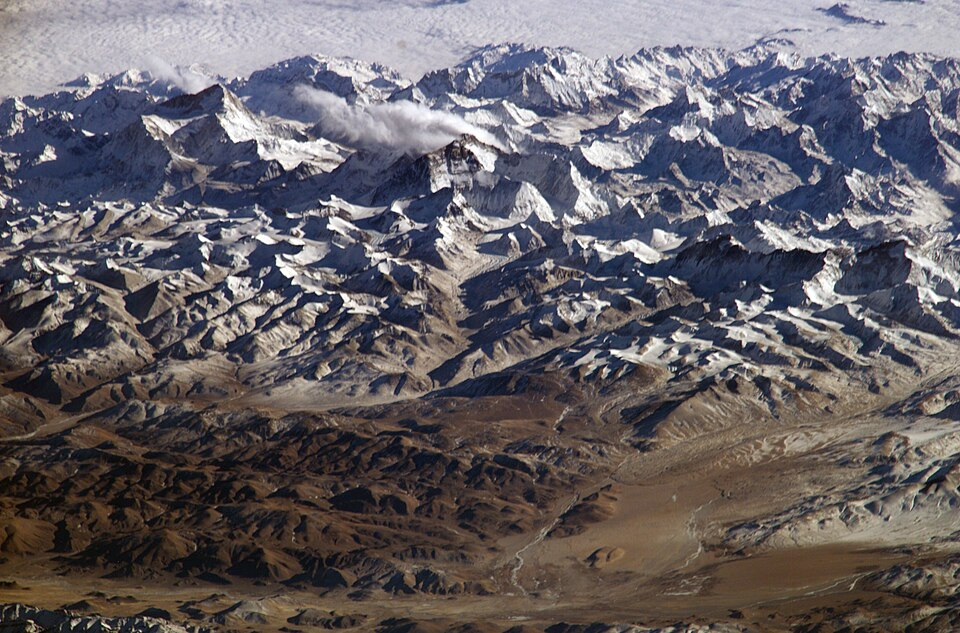
\includegraphics[width=0.75\linewidth]{images/book1/g4-himalaya-iss.jpg}

{\small The Himalaya seen from the International Space Station, looking
south from the high plateau of Tibet: a sea of snow-covered summits.
Photograph: NASA (public domain).}
% ledger: nasa:himalaya-iss
\end{omfigure}

\section{The great rivers and lakes}

\omterm{def:g4:clouds-rain-snow:precipitation}{Rain} and melted \omterm{def:g4:clouds-rain-snow:precipitation}{snow} run off the land, join into streams and then into
\omterm{def:g1:landscapes-around-us:water}{rivers}, and the \omterm{def:g1:landscapes-around-us:water}{rivers} carry the water down to the \omterm{def:g2:water-on-earth:ocean}{sea}. The largest \omterm{def:g1:landscapes-around-us:water}{rivers}
drain whole regions of a \omterm{def:g3:continents-and-oceans:continent}{continent}.

The two longest \omterm{def:g1:landscapes-around-us:water}{rivers} on Earth are the Nile, in Africa, and the Amazon, in
South America. Each is close to 7\,000 kilometres long. Which one is the
longest? Nobody agrees for sure, because it depends on where you decide
that a \omterm{def:g1:landscapes-around-us:water}{river} starts: among all the little streams that join to make it,
which one counts as its true beginning? In 2007, a team that followed the
Amazon to a farther source said it was about 6\,800 kilometres long, a
little longer than the Nile; many reference books still call the Nile the
longest.
% ledger: natgeo:nile, natgeo:amazon-nile-2007

The Amazon is, without any doubt, the largest \omterm{def:g1:landscapes-around-us:water}{river}: it carries more water
than any other.
% ledger: natgeo:amazon-nile-2007

\begin{omfigure}
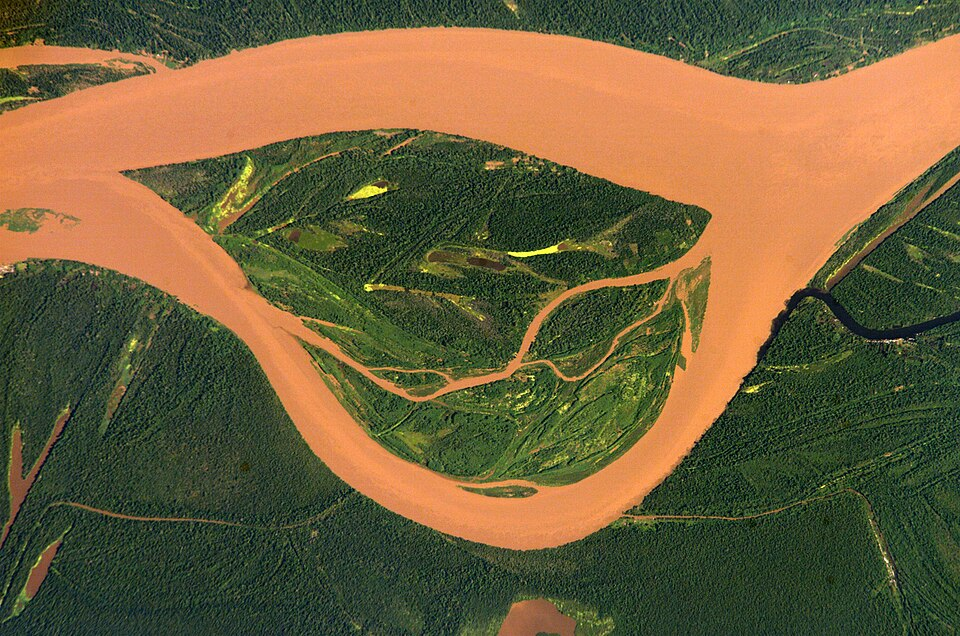
\includegraphics[width=0.6\linewidth]{images/book1/g4-amazon-iss.jpg}

{\small The Amazon, brown with \omterm{def:g3:stones-pebbles-sand:sand}{mud}, winding through the rainforest, seen
from the International Space Station. Photograph: NASA (public domain).}
% ledger: nasa:amazon-iss
\end{omfigure}

\omterm{def:g1:landscapes-around-us:water}{Lakes} also break records. The largest \omterm{def:g1:landscapes-around-us:water}{lake} on Earth is the Caspian Sea,
between Europe and Asia: it is so big that it is called a \omterm{def:g2:water-on-earth:ocean}{sea}, but it is
closed in by land on every side. It covers more than
370\,000 square kilometres. The deepest \omterm{def:g1:landscapes-around-us:water}{lake} is \omterm{def:g1:landscapes-around-us:water}{Lake} Baikal, in Russia: in
places its bottom lies nearly 2 kilometres below its surface.
% ledger: natgeo:caspian-baikal

\section{Deserts and the great ice}

Two kinds of places stand out on the \omterm{def:g4:world-physical-map:physical-map}{physical map} because almost nothing
grows there: the great deserts, where it almost never \omterm{def:g4:clouds-rain-snow:precipitation}{rains}, and the great
ice.

The Sahara, in the north of Africa, is the largest hot desert on Earth. It
covers about eight and a half million square kilometres. Africa as a whole
covers about 30 million square kilometres, so the Sahara is a little more
than a quarter of the \omterm{def:g3:continents-and-oceans:continent}{continent}: more than $\frac{1}{4}$, but less than
$\frac{1}{3}$.
% ledger: natgeo:sahara, data:etopo1

The great ice covers Antarctica, around the \omterm{def:g3:continents-and-oceans:poles}{South Pole}, and most of
Greenland, in the far north of the Atlantic. There, the \omterm{def:g4:clouds-rain-snow:precipitation}{snow} of thousands of
years has piled up and turned into a thick layer of ice. On the \omterm{def:g4:world-physical-map:physical-map}{physical map}, their colours are those of high
land, because the top of the ice is high above \omterm{def:g4:world-physical-map:altitude}{sea level}.

\section{The highest and the deepest}

The \omterm{def:g4:world-physical-map:physical-map}{physical map} shows the shape of the Earth's surface, but it is so
small that it hides the extremes. Let us put them side by side, to scale.

\begin{omfigure}
\begin{tikzpicture}[x=1cm, y=0.32cm, font=\small]
  % sea level
  \fill[omHypsSeaA] (0,0) rectangle (9,-11.5);
  \fill[omHypsSeaD!80] (4.6,-11.5) -- (4.6,-11.0) -- (5.0,-10.98) -- (5.4,-11.0) -- (5.4,-11.5) -- cycle;
  \draw[black!60] (-0.2,0) -- (9.2,0);
  \node[anchor=west, font=\scriptsize] at (9.25,0) {sea level, 0\,m};
  % height scale
  \draw[black!60] (0,-11.5) -- (0,10);
  \foreach \h in {-10,-8,...,8} {
    \draw[black!60] (-0.1,\h) -- (0,\h);
    \node[anchor=east, font=\scriptsize] at (-0.12,\h) {\h\,km};
  }
  % ocean floor and trench
  \fill[brown!45] (0.05,-11.5) -- (0.05,-3.7) -- (3.2,-3.7) -- (4.4,-6) -- (4.9,-10.98) -- (5.1,-10.98)
    -- (5.6,-6) -- (6.4,-3.7) -- (9,-3.7) -- (9,-11.5) -- cycle;
  \node[font=\scriptsize, align=center] at (2.0,-5.3) {ocean floor,\\about 3\,700\,m deep};
  \node[font=\scriptsize, anchor=west, align=left] at (5.6,-9.4) {the deepest point:\\Challenger Deep,\\nearly 11\,000\,m};
  % Everest
  \fill[black!35] (6.6,0) -- (7.6,8.85) -- (8.6,0) -- cycle;
  \fill[white, draw=black!45, line width=0.3pt] (7.35,6.6) -- (7.6,8.85) -- (7.85,6.6) -- (7.6,7.1) -- cycle;
  \node[font=\scriptsize, align=center, anchor=south] at (7.6,8.95) {Mount Everest, 8\,849\,m};
  % cirrus clouds band
  \draw[black!45, line width=0.6pt] (1.0,9.0) .. controls (1.6,9.5) and (2.2,9.1) .. (2.8,9.6);
  \draw[black!45, line width=0.6pt] (1.2,8.3) .. controls (1.8,8.8) and (2.4,8.4) .. (3.0,8.9);
  \node[font=\scriptsize, align=center] at (2.0,7.2) {high clouds\\(cirrus)};
  % a village
  \fill[black!60] (2.2,1.5) rectangle (2.45,1.75);
  \node[font=\scriptsize, anchor=west] at (2.5,1.6) {a mountain village, 1\,500\,m};
\end{tikzpicture}

{\small From the deepest point of the \omterm{def:g2:water-on-earth:ocean}{ocean} to the highest summit, to
scale. The Challenger Deep, in the Pacific \omterm{def:g2:water-on-earth:ocean}{Ocean}, lies deeper below the
\omterm{def:g2:water-on-earth:ocean}{sea} than Mount Everest rises above it. Values: Everest 8\,849\,m; the
Challenger Deep nearly 11\,000\,m; the average \omterm{def:g2:water-on-earth:ocean}{ocean} floor about
3\,700\,m.}
\label{fig:g4:world-physical-map:extremes}
% ledger: tht:everest, usgs:trench-depth, nos:ocean-depth, wmo:cloud-levels
\end{omfigure}

\begin{example}[Everest in the deep]\label{ex:g4:world-physical-map:everest-in-deep}
If we could lift Mount Everest and set it down at the bottom of the
Challenger Deep, its summit would still be under the water: about 11\,000
metres of trench, against 8\,849 metres of \omterm{def:g1:landscapes-around-us:landform}{mountain}. More than 2
kilometres of \omterm{def:g2:water-on-earth:ocean}{sea} would still cover it.
% ledger: tht:everest, usgs:trench-depth
\end{example}

\section{Exercises}

\begin{exercise}[$\star$]\label{exo:g4:world-physical-map:1}
What is the \omterm{def:g4:world-physical-map:altitude}{altitude} of a place? From which level is it measured?
\end{exercise}

\begin{exercise}[$\star$]\label{exo:g4:world-physical-map:2}
Using the \omterm{def:g2:drawing-to-map:legend}{legend} of the \omterm{def:g4:world-physical-map:physical-map}{physical map}, give the \omterm{def:g4:world-physical-map:altitude}{altitude} of a place
coloured: (a) dark green; (b) pale yellow; (c) almost white.
\end{exercise}

\begin{exercise}[$\star$]\label{exo:g4:world-physical-map:3}
On which \omterm{def:g3:continents-and-oceans:continent}{continent} is: (a) the Andes; (b) the Himalaya; (c) the Sahara;
(d) the Rocky \omterm{def:g1:landscapes-around-us:landform}{Mountains}?
\end{exercise}

\begin{exercise}[$\star$]\label{exo:g4:world-physical-map:4}
Name the highest \omterm{def:g1:landscapes-around-us:landform}{mountain} on Earth, the largest \omterm{def:g1:landscapes-around-us:water}{lake} and the deepest \omterm{def:g1:landscapes-around-us:water}{lake}.
\end{exercise}

\begin{exercise}[$\star$]\label{exo:g4:world-physical-map:5}
On the \omterm{def:g4:world-physical-map:physical-map}{physical map}, the \omterm{def:g2:water-on-earth:ocean}{sea} near the \omterm{def:g1:landscapes-around-us:water}{coasts} is pale blue and the middle of
the \omterm{def:g2:water-on-earth:ocean}{oceans} dark blue. What does that tell you about the depth of the \omterm{def:g2:water-on-earth:ocean}{sea}?
\end{exercise}

\begin{exercise}[$\star$]\label{exo:g4:world-physical-map:6}
Why are Antarctica and Greenland coloured like high land on the \omterm{def:g4:world-physical-map:physical-map}{physical
map}?
\end{exercise}

\begin{exercise}[$\star\star$]\label{exo:g4:world-physical-map:7}
Put in order, from the lowest to the highest: a beach; a village at
1\,500 metres; the top of Mount Everest; the bottom of the Challenger
Deep; the average floor of the \omterm{def:g2:water-on-earth:ocean}{ocean}.
\end{exercise}

\begin{exercise}[$\star\star$]\label{exo:g4:world-physical-map:8}
Why can't we say for sure whether the Nile or the Amazon is the longest
\omterm{def:g1:landscapes-around-us:water}{river}?
\end{exercise}

\begin{exercise}[$\star\star$]\label{exo:g4:world-physical-map:9}
Africa covers about 30 million square kilometres. Which part of it is a
quarter? A third? The Sahara covers about eight and a half million square
kilometres: is it more or less than a quarter of Africa? More or less than
a third?
\end{exercise}

\begin{exercise}[$\star\star$]\label{exo:g4:world-physical-map:10}
A \omterm{def:g1:landscapes-around-us:landform}{mountain} hut stands at 2\,500 metres, and a \omterm{def:g1:landscapes-around-us:water}{lake} below it at 1\,000
metres. How many metres higher is the hut? Which colours do they have on
the \omterm{def:g4:world-physical-map:physical-map}{physical map}?
\end{exercise}

\begin{exercise}[$\star\star\star$]\label{exo:g4:world-physical-map:11}
A plane flies 10 kilometres above \omterm{def:g4:world-physical-map:altitude}{sea level}. Is it higher than Mount
Everest? By how many metres? If it flew over the Challenger Deep, how far
above the bottom of the trench would it be (take 11\,000 metres for the
trench)?
\end{exercise}
